\documentclass{article}
\usepackage[a4paper, total={7.5in, 10in}]{geometry}
\geometry{paperwidth=8in, paperheight=16383pt, left=1in, top=40pt, textwidth=6in, marginparsep=20pt, marginparwidth=100pt, textheight=16263pt, footskip=40pt}
\usepackage{graphicx}
\usepackage{url}
\usepackage{natbib}
\usepackage{todonotes}
\usepackage{booktabs}
\usepackage{lineno}
\usepackage{color}
%\usepackage{auto-pst-pdf}
\usepackage[colaction]{multicol}
\usepackage{caption}
\usepackage{svg}
\usepackage{authblk}
\usepackage{standalone}
\usepackage[section]{placeins}


\linespread{1.5}

\makeatletter
\renewcommand{\maketitle}{\bgroup\setlength{\parindent}{0pt}
	\begin{flushleft}

		{\huge\textbf{\@title}}

		\bigskip

 		{\large\textbf{\@author}}

 		\bigskip

 		{\large{Draft current \@date}}

	\end{flushleft}\egroup
}
\makeatother

\newcommand{\multicollinenumbers}{
	\linenumbers
	\def\makeLineNumber{\docolaction
		{\makeLineNumberLeft}
		{}
		{\makeLineNumberRight}
		}
}

\newenvironment{figurehere}
	{\def\@captype{figure}}
	{}

% Title
\title{A Topic Model of Climate Change Literature}
\title{Words, words, words: Mapping the Matter of Climate Change Literature}
\title{A Topography of Climate Change Research - Results}
\author[1,2]{Max Callaghan}

\affil[1]{Mercator Research Institute on Global Commons and Climate Change, Torgauer Straße, 10829 Berlin, Germany}
\affil[2]{School of Earth and Environment, University of Leeds, Leeds LS2 9JT, United Kingdom}

\begin{document}
\maketitle

\section{Results}

\setcounter{totalnumber}{200}

	
\begin{table}[h]
	\scriptsize
	\begin{tabular}{|l |p{1.8cm} p{1.8cm} p{1.8cm} p{1.8cm} p{1.8cm} p{1.8cm}|} 
\hline 
&\textbf{AR1} & \textbf{AR2} & \textbf{AR3} & \textbf{AR4} & \textbf{AR5} & \textbf{AR6}\\ \hline
	\caption{Growth in climate change literature}
	\label{growthtable}
\end{table}

\begin{figure}[h]
	\begin{center}
		\includegraphics[width=0.5\linewidth]{plots/literature_size/volume_variety.pdf}
		%\captionof{figure}
		\caption{The volume and variety of literature on climate change has grown to unmanageable proportions. Each box represents a document-term matrix (unique documents x unique terms) of the abstracts written in each assessment period. The percentage of documents in which the average word occurs in is given in the key.
		}
	
		\label{growth}
	\end{center}
\end{figure}

\begin{figure}[h]
	\begin{center}
		%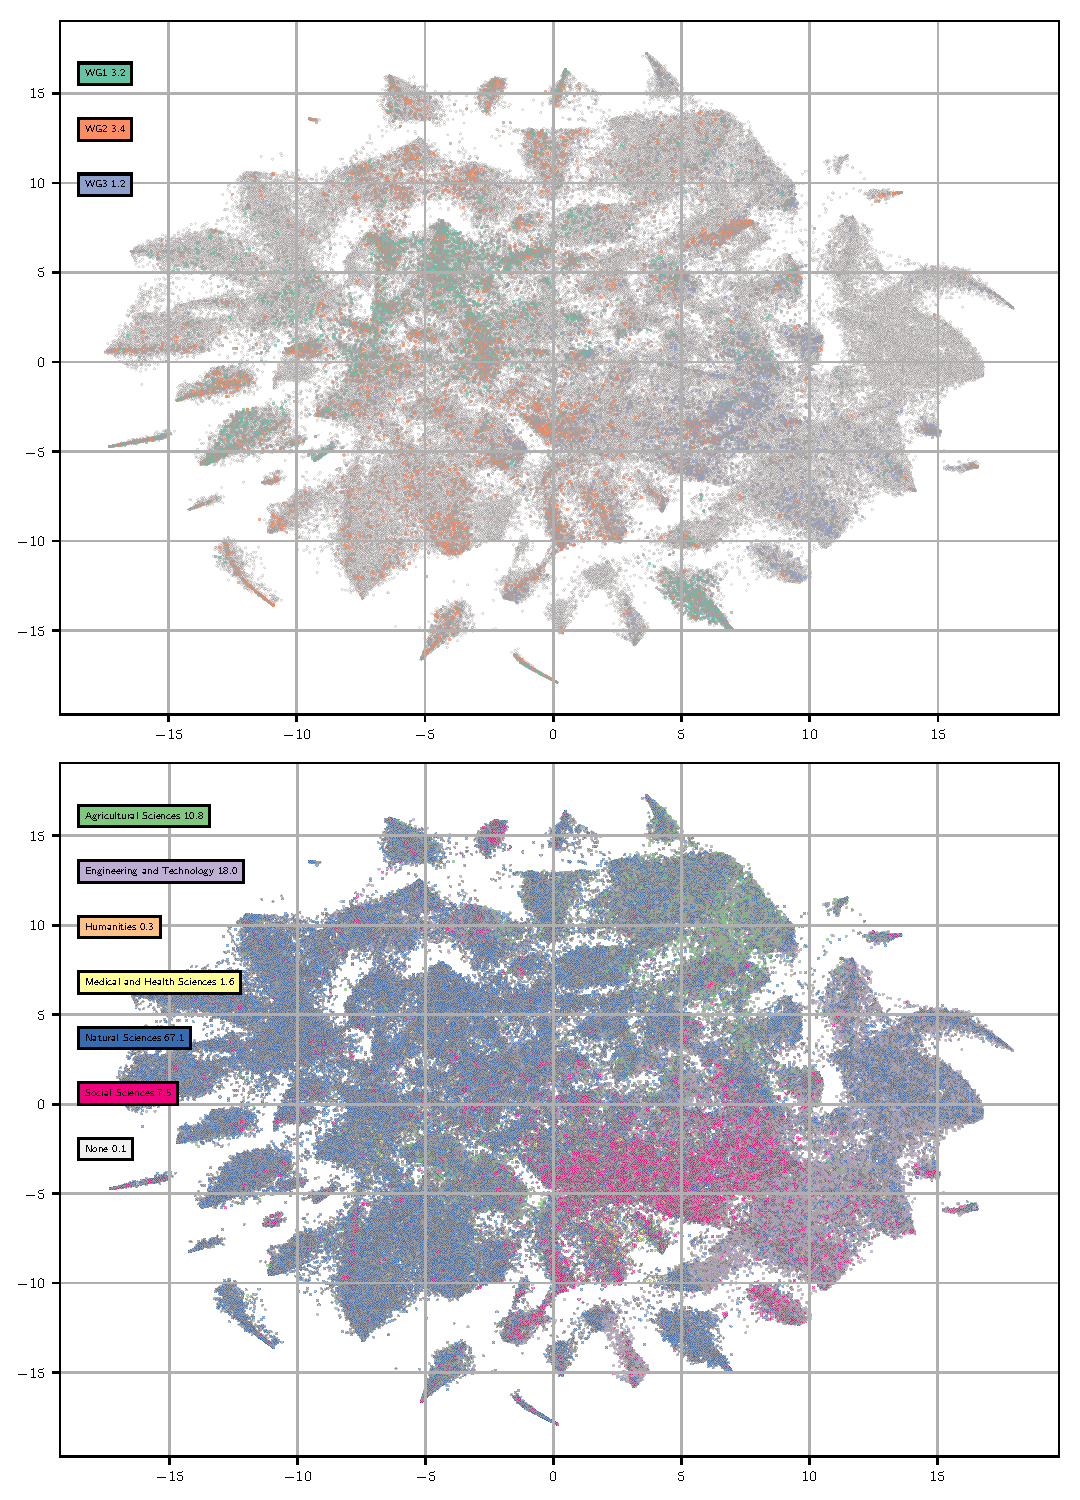
\includegraphics[width=1\linewidth]{tsne_results/plots/run_665_s_0_p200_double.pdf}
		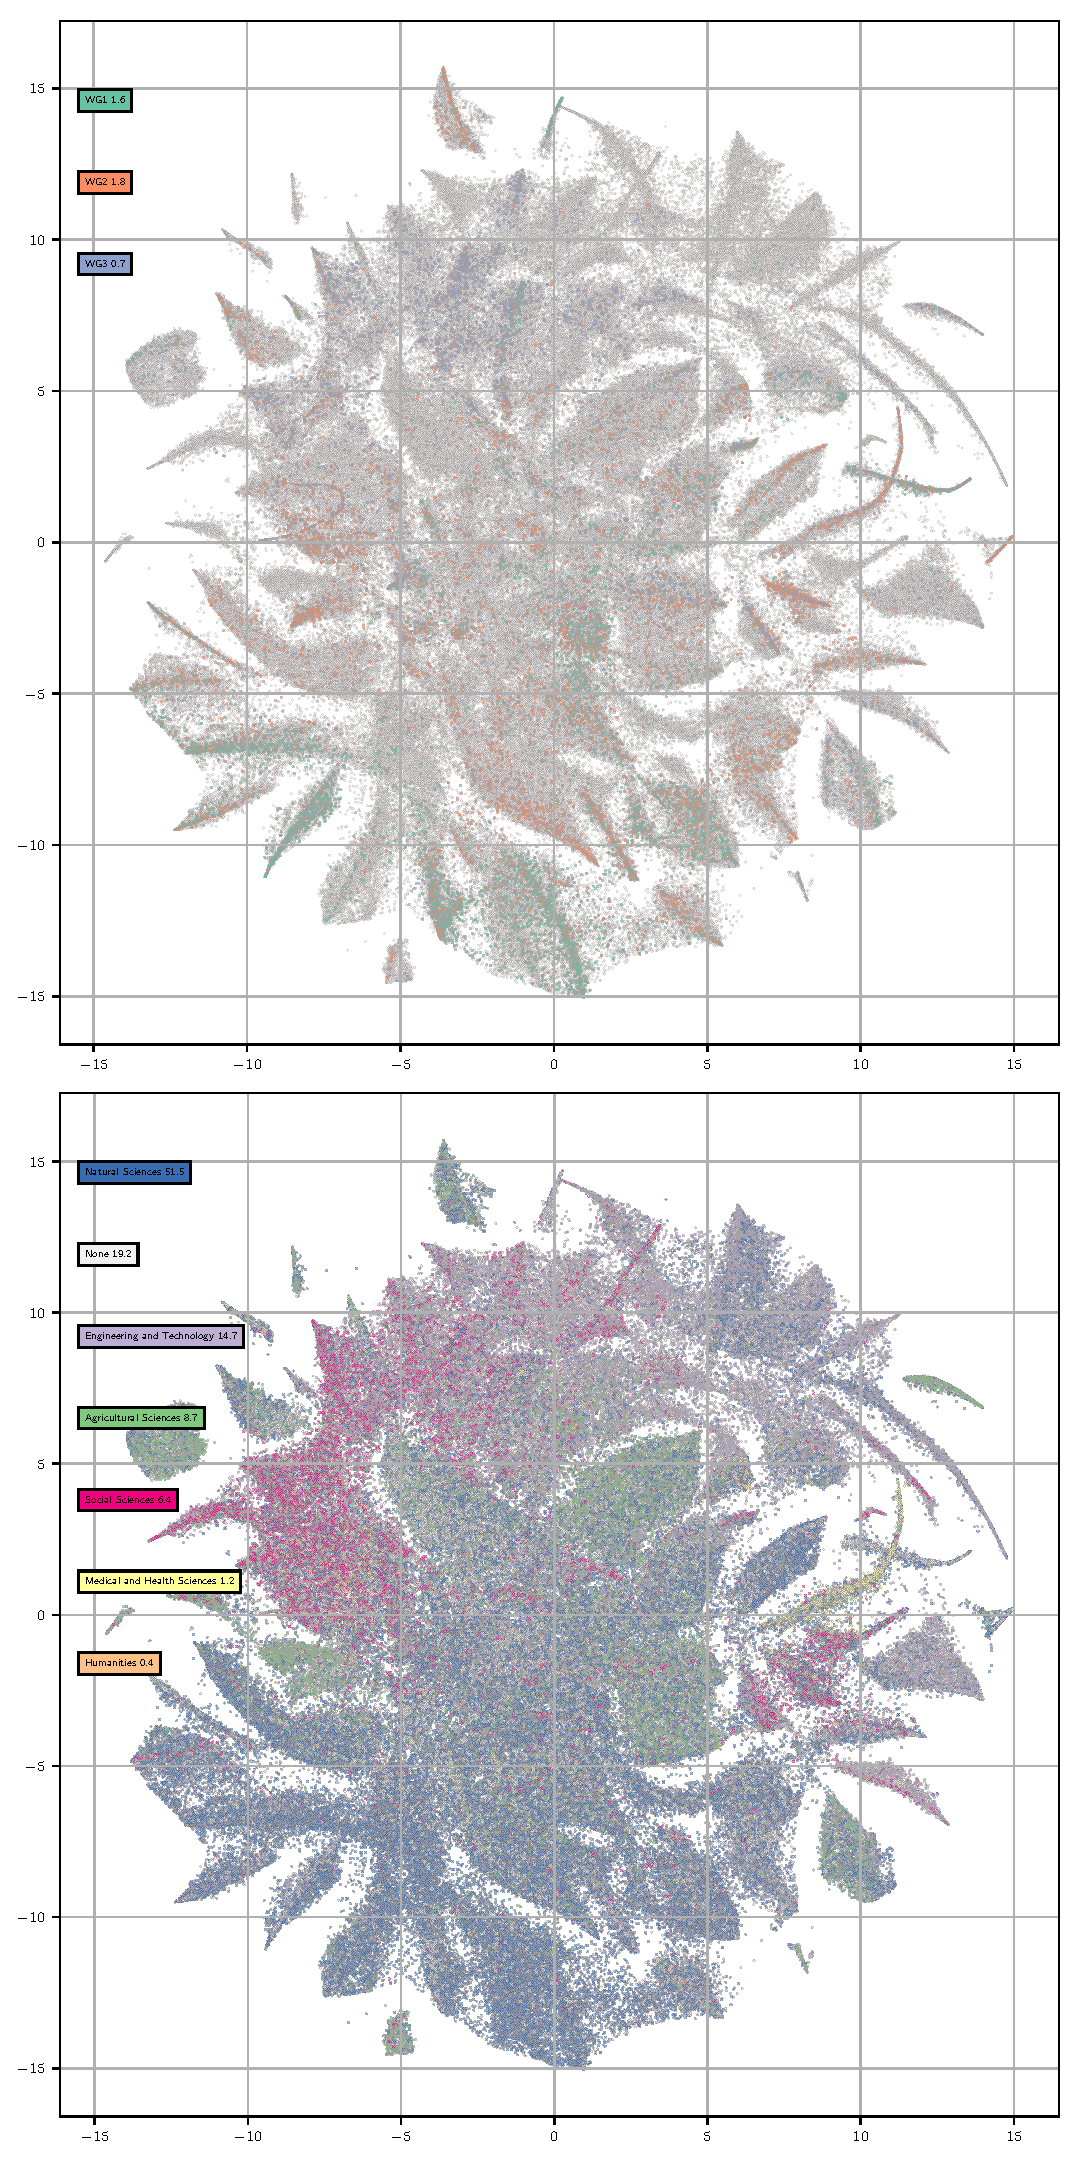
\includegraphics[width=0.85\linewidth]{tsne_results/plots/run_1275_s_0_p100_double.png}
		\caption{A map of the literature on climate change. Document positions are obtained by reducing the topic scores to two dimensions via t-SNE Documents are coloured by working group citations (top) and web of science discipline category (bottom). See SI table for topic composition of each grid square}
		\label{map-double}
	\end{center}
\end{figure}

\begin{figure}[h!]
	\begin{center}
		\includegraphics[width=0.85\linewidth]{plots/ipcc_representation/ipcc_rep_oecds_time.pdf}
		\caption{A map of the literature on climate change. Document positions are obtained by reducing the topic scores to two dimensions via t-SNE Documents are coloured by working group citations (top) and web of science discipline category (bottom). See SI table for topic composition of each grid square}
		\label{oecd_rep}
	\end{center}
\end{figure}

\begin{figure}[h!]
	\begin{center}
		%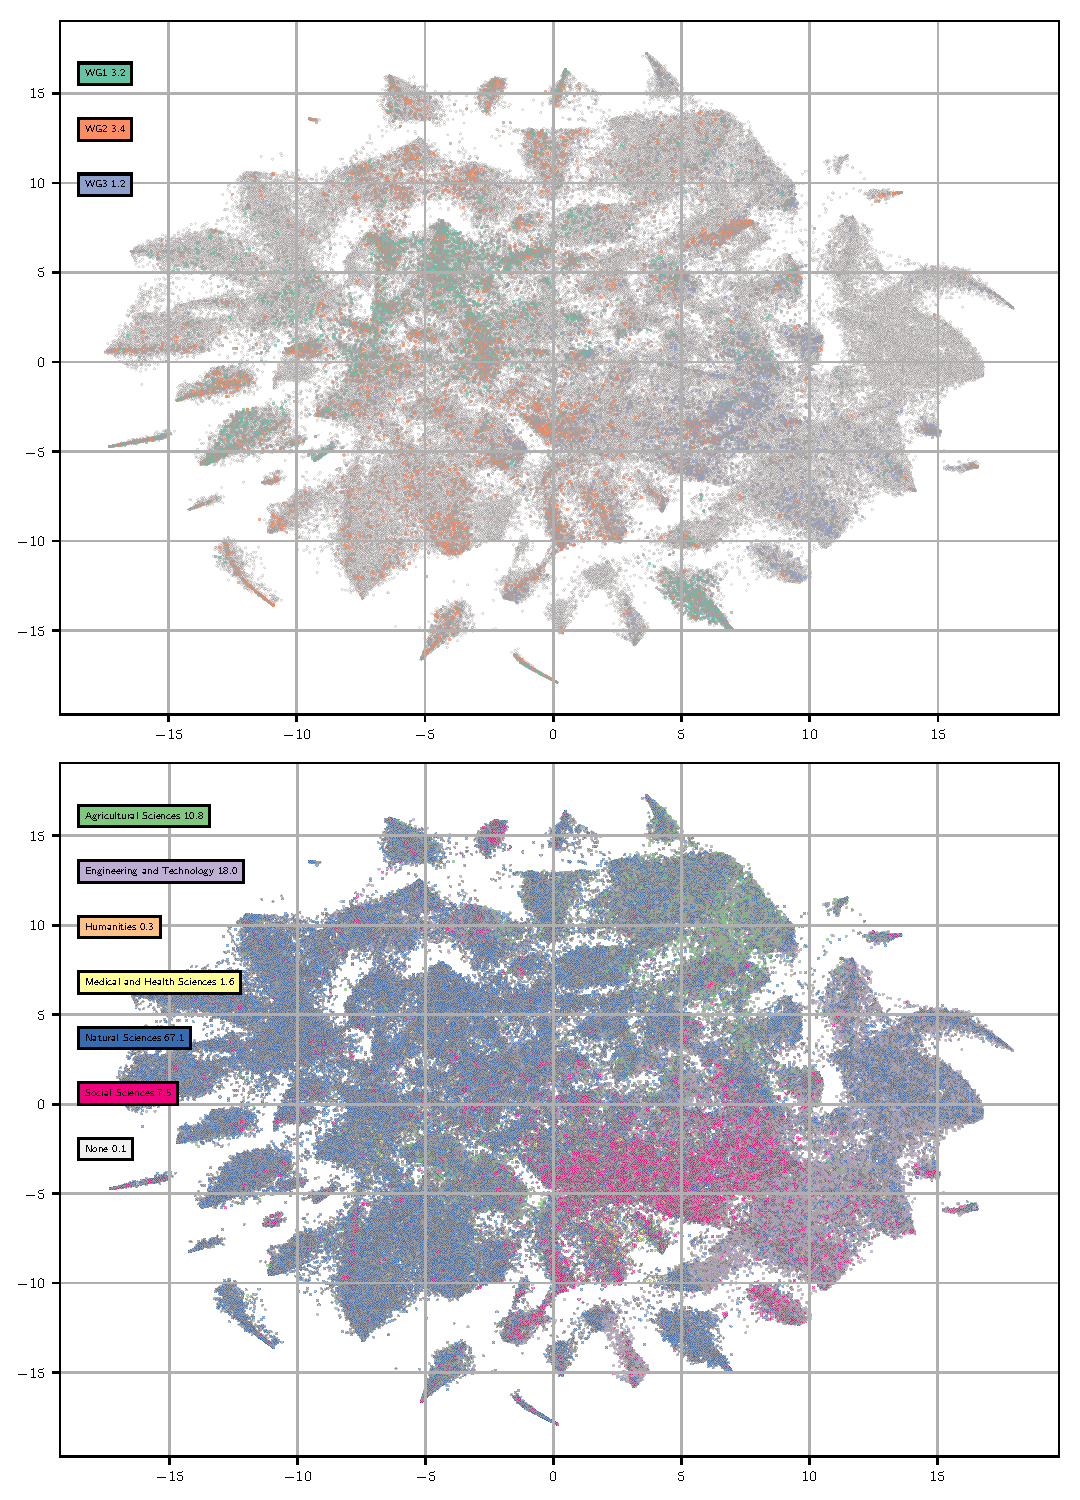
\includegraphics[width=1\linewidth]{tsne_results/plots/run_665_s_0_p200_double.pdf}
		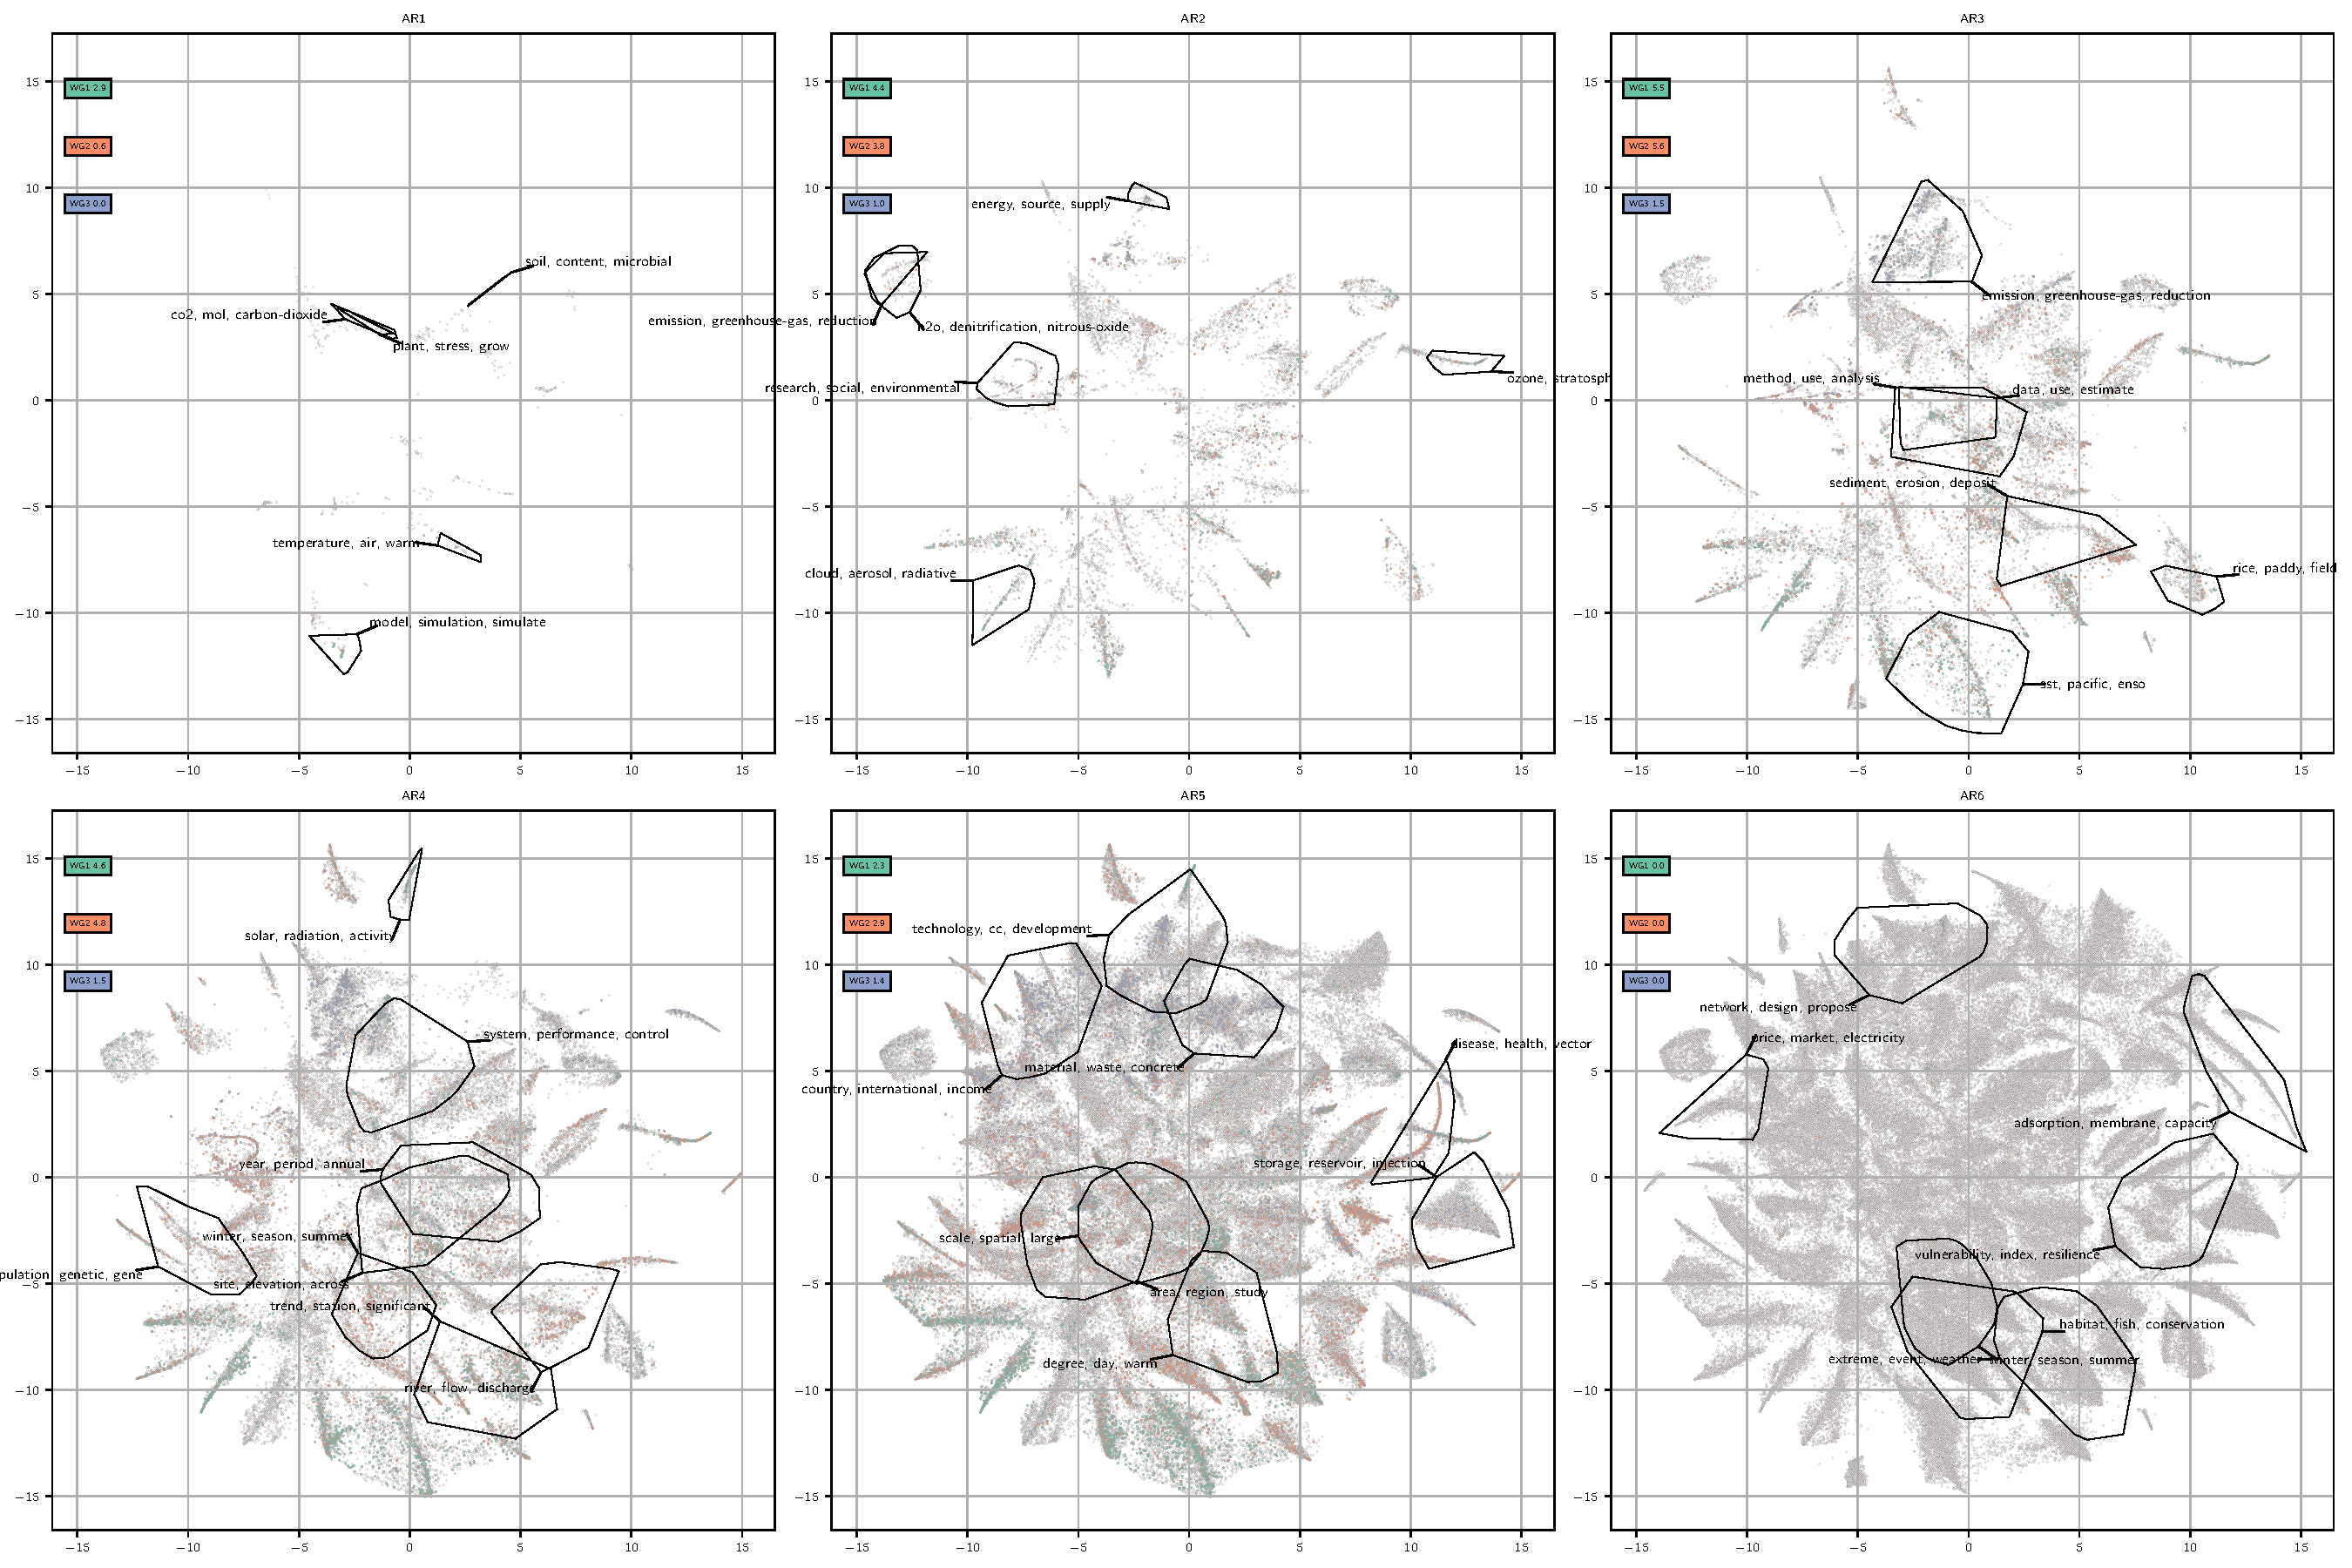
\includegraphics[width=1\linewidth]{tsne_results/plots/run_1275_s_0_p100_evolution.png}
		\caption{A map of the literature on climate change. Document positions are obtained by reducing the topic scores to two dimensions via t-SNE Documents are coloured by working group citations (top) and web of science discipline category (bottom). See SI table for topic composition of each grid square}
		\label{map-double}
	\end{center}
\end{figure}


\begin{figure}[h!]
	\begin{center}
		\includegraphics[width=0.85\linewidth]{plots/ipcc_representation/ipcc_rep_new1275_all.pdf}
		\caption{A map of the literature on climate change. Document positions are obtained by reducing the topic scores to two dimensions via t-SNE Documents are coloured by working group citations (top) and web of science discipline category (bottom). See SI table for topic composition of each grid square}
		\label{ipcc_rep}
	\end{center}
\end{figure}




\begin{table}[h!]
	\scriptsize
	\begin{tabular}{p{1.9cm} p{3cm} p{7.5cm} r}
\toprule
                      title &                                                                            top words &                                                                                                                                                                                                                                                                top docs &   share \\
\midrule
      climat, chang, impact &          [climat, chang, impact, respons, futur, effect, shift, sensit, affect, may] &                                                                                                                                                  \parbox[t]{7.5cm}{Climate oscillations and changes over Russia; \\World Regionalization of Climate Change (1961-2010)} &  2.73\% \\
     soil, moistur, microbi &       [soil, moistur, microbi, organ, respir, content, miner, depth, matter, efflux] &                                                                                    \parbox[t]{7.5cm}{PARTITIONING OF SOIL RESPIRATION IN A FIRST ROTATION BEECH PLANTATION; \\Responses of soil respiration to N fertilization in a loamy soil under maize cultivation} &  2.73\% \\
       emiss, reduct, reduc &      [emiss, reduct, reduc, greenhous, factor, total, estim, inventori, nox, measur] &                                                                                                             \parbox[t]{7.5cm}{China's CH4 and CO2 emissions: Bottom-up estimation and comparative analysis; \\Monitoring total emissions from industrial installations} &  2.21\% \\
   carbon, dioxid, sequestr &   [carbon, dioxid, sequestr, sink, organ, cycl, storag, stock, terrestri, atmospher] &                             \parbox[t]{7.5cm}{Interpreting carbon-isotope excursions: carbonates and organic matter; \\PARTICULATE FLUXES OF CARBONATE AND ORGANIC-CARBON IN THE OCEAN - IS THE MARINE BIOLOGICAL-ACTIVITY WORKING AS A SINK OF THE ATMOSPHERIC CARBON} &  1.74\% \\
      temperatur, air, mean &  [temperatur, air, mean, surfac, minimum, maximum, daili, increas, effect, degreesc] &                                                                                                     \parbox[t]{7.5cm}{Observed changes in shallow soil temperatures in Northeast China, 1960-2007; \\Beyond the Mean: Biological Impacts of Cryptic Temperature Change} &  1.71\% \\
      record, dure, glacial &       [record, dure, glacial, reconstruct, last, period, holocen, event, late, core] &                                                           \parbox[t]{7.5cm}{HIGH-RESOLUTION CLIMATE RECORDS FROM THE NORTH-ATLANTIC DURING THE LAST INTERGLACIAL; \\HIGH-RESOLUTION CLIMATIC INFORMATION FROM SHORT FIRN CORES, WESTERN DRONNING MAUD LAND, ANTARCTICA} &   1.7\% \\
     speci, distribut, rang &          [speci, distribut, rang, rich, invas, nich, predict, extinct, shift, abund] &                               \parbox[t]{7.5cm}{Northward range extensions of some mesopelagic fishes in the Northeastern Atlantic; \\Natural occurrence and backwater infection of C-4 plants in the vegetation of the Yangtze hydropower Three Gorges Project region} &   1.7\% \\
 increas, concentr, decreas &   [increas, concentr, decreas, effect, atmospher, doc, result, organ, nutrient, may] &                                                          \parbox[t]{7.5cm}{TERRESTRIAL HIGHER-PLANT RESPONSE TO INCREASING ATMOSPHERIC [CO2] IN RELATION TO THE GLOBAL CARBON-CYCLE; \\Hydrological response to climate change in the Black Hills of South Dakota, USA} &  1.61\% \\
      forest, tropic, stand &       [forest, tropic, stand, deforest, disturb, stock, boreal, redd, harvest, wood] &  \parbox[t]{7.5cm}{Spatially explicit estimates and temporal changes of forest tree biomass in a typical department of forest management, Turkey; \\Analysis of the changes in forest ecosystem functions, structure and composition in the Black Sea region of Turkey} &  1.56\% \\
    energi, renew, consumpt &        [energi, renew, consumpt, effici, demand, save, sector, sourc, industri, use] &                                                                                                                                       \parbox[t]{7.5cm}{Energy issues and energy priorities; \\Energy efficiency and CO2 emissions in Swedish manufacturing industries} &  1.56\% \\
\bottomrule
\end{tabular}

	\caption{Top 10 topics in climate change literature}
	\label{top-topics}
\end{table}	

\end{document}